\documentclass{beamer}

\usepackage[utf8x]{inputenc} % can be changed to utf8x
\usepackage[T1]{fontenc}
\usepackage[french]{babel}
\usepackage{lmodern}
\usepackage{color}
\usepackage{listings}
\usepackage{svg}
\usepackage{appendixnumberbeamer}
\usepackage{hyperref}


\usepackage{booktabs}
\usepackage[scale=2]{ccicons}

\usepackage{pgfplots}
\usepgfplotslibrary{dateplot}

\usepackage{xspace}
\newcommand{\themename}{\textbf{\textsc{metropolis}}\xspace}
\definecolor{orange}{rgb}{1,0.5,0}

\lstdefinelanguage{python}
{morekeywords=[1]{import,from,False,True,and,or,not,if,else,elif,while,break,continue,def,return,global,in,None,for,class,is,try,except,pass,assert,lambda,raise,yield,nonlocal,with,as,cdef,extern},
morekeywords=[2]{complex,str,int,set,dict,frozenset,list,float},
morekeywords=[3]{print,type,sqrt,input,sin,len,del,range,namedtuple,radians,chr,isinstance,zip,map,filter,sum,all,any,iter,next,callable,open},
morekeywords=[4]{@property},
morekeywords=[5]{OSError,StopIteration,IndexError,ValueError,IOError},
morestring=[b]{"},
morestring=[b]{'},
morestring=[b]{"""},
morecomment=[l]{\#},}[keywords,comments,strings,directives]

% Listing style
\lstset{basicstyle=\fontsize{7}{8}\selectfont\tt}
\lstset{keywordstyle=[1]\color[rgb]{0,0,1}\bfseries}
\lstset{keywordstyle=[2]\color[rgb]{0.6,0,0}\bfseries}
\lstset{keywordstyle=[3]\color[rgb]{0,0.6,0}\bfseries}
\lstset{keywordstyle=[4]\color{orange}\bfseries}
\lstset{keywordstyle=[5]\color[rgb]{0.463,0.294,0.557}\bfseries}
\lstset{directivestyle=\color[rgb]{0.314,0.40,0.565}\bfseries}
\lstset{identifierstyle=\color{black}}
\lstset{commentstyle=\color[rgb]{0,0.6,0.6}}
\lstset{stringstyle=\color[rgb]{0.44,0.47,1}}
\lstset{stringstyle=\color[rgb]{0.44,0.47,1}}
\lstset{showstringspaces=false,showtabs=false,tabsize=3,extendedchars=true,breaklines=true,postbreak={},breakautoindent=true,breakindent=0pt}
\lstset{frame=shadowbox,rulecolor=\color[gray]{.2},rulesepcolor=\color[gray]{.75},framesep=2pt,backgroundcolor=\color[rgb]{1,1,0.9}}
\lstset{xleftmargin=0.1cm,xrightmargin=1mm,aboveskip=0.5cm,belowskip=0cm}
\lstset{captionpos=b,numbers=left,numberstyle=\tiny,columns=fixed,escapechar=§}
\lstset{language=python}

\usetheme{metropolis}           % Use metropolis theme
\title{Design Pattern: Strat\'egie}
\date{\today}
\author{Jonathan Petit}
\institute{ECAM - Architecture logicielle}
\begin{document}
  \maketitle

\section{Design Pattern: Strat\'egie}

  \begin{frame}{Introduction}
    \frametitle{Introduction}
    \begin{itemize}
      \item  \textcolor{red}{Design pattern} \\
      \textit{Mod\`ele de conception pour une solution reproductible à un probl\`eme r\'ecurrent}
      \item Accélère le processus de dévellopement en fournissant un \textcolor{red}{modèle} testé et approuvé. \\
      \item 3 catégories \\ \textit{\textcolor{red}{Structurelle}, \textcolor{red}{ Comportementale} et de  \textcolor{red}{Création}} 
    \end{itemize}
  \end{frame}

  \begin{frame}{Le design pattern stratégie}
    \frametitle{Le design pattern stratégie}
    \begin{itemize}
      \item Design pattern \textcolor{red}{Comportemental} \\
      \textit{Encapsule une famille d'algorithme dans une classe.}
      \item \textcolor{red}{Idépendance} du client utilisateur \\
      \textit{L'algorithme varie en fonction de l'utilisation d'un client}
      \item Cache les \textcolor{red}{details d'implémentation} \\
      \textit{Grâce à une abstraction réaliser dans une interface.}
    \end{itemize}
  \end{frame}
  
    \begin{frame}{Utilisation}
    \frametitle{Utilisation}
    \begin{itemize}
      \item Plusieurs \textcolor{red}{choix} d'algorithme  \\
      \textit{Quand un classe a différents choix d'algorithmes.}
      \item Plusieurs \textcolor{red}{procédures} \\
      \textit{Quand une même tâche a plusieurs algorithmes.}
    \end{itemize}
  \end{frame}

  \begin{frame}{Structure (1)}
    \frametitle{Structure (1)}
    \begin{itemize}
      \item Une interface
      \item Plusieurs implémentation de l'interface (les stratégies)
      \item Un contexte
      \item Un client
    \end{itemize}
    \begin{figure}[!b]
      \centering
      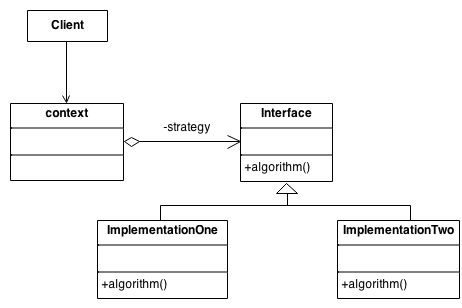
\includegraphics[scale=0.27]{Strategy}
      \caption{Structure: design pattern stratégie}
    \end{figure}
  \end{frame}
  
    \begin{frame}{Structure (2)}
    \frametitle{Structure (2)}
    \begin{itemize}
      \item \textcolor{red}{Encapsulation} de l'interface \\
      \textit{Les détails d'implémentation sont alors cacher dans les classes d'implémentation de l'interface.}
      \item \textcolor{red}{Aucun} impact sur le client \\
      \textit{Si l'implémentation des stratégies changent.}
    \end{itemize}
        \lstinputlisting[firstline=0,lastline=5]{interface.py}
  \end{frame}

  \begin{frame}{L'interface}
    \frametitle{L'interface}
    \begin{itemize}
      \item L'interface avec les différentes \textcolor{red}{abstractions} \\
      \textit{Les algorithmes représentant les différentes stratégies implémenteront les méthodes abstraites.}
    \end{itemize}
        \lstinputlisting[firstline=0,lastline=5]{interface.py}
  \end{frame}

  \begin{frame}{Les stratégies}
    \frametitle{Les stratégies}
    \begin{itemize}
      \item Les différentes \textcolor{red}{algorithmes} stratégies  implémente l'interface \\
      \textit{Les statégies implémente les méthodes de l'interface afin de cacher les détails aux utilisateurs.}
    \end{itemize}
    \lstinputlisting[firstline=0,lastline=15]{implementation.py}
  \end{frame}

  \begin{frame}{Le contexte}
    \frametitle{Le contexte}
    \begin{itemize}
      \item Le contexte \textcolor{red}{dirige} les clients \\
      \textit{Redirection par l'interface vers les différentes stratégies.}
    \end{itemize}
    \lstinputlisting[firstline=0,lastline=15]{context.py}
  \end{frame}
  
    \begin{frame}{Exemple d'utilisation}
    \frametitle{Exemple d'utilisation}
    \begin{itemize}
      \item Application de \textcolor{red}{payements} \\
      \textit{Plusieurs moyen de payments, par carte, en cash, ...}
      \item Application de \textcolor{red}{trajet} \\
      \textit{Un client peut choisir de faire un tajet en bus, en train, en voiture, ...}
    \end{itemize}
  \end{frame}

    \begin{frame}{Application (1)}
    \frametitle{Application (1): Description}
    \begin{itemize}
      \item \textcolor{red}{"Tout le monde veut prendre ça place"} \\
      \textit{Application basique du jeu télévisé.}
      \item Plusieurs \textcolor{red}{procédures} de réponses \\
      \textit{Un participant peut choisir entre plusieurs méthodes de réponse (DUO, CARRE ou CASH.)}
        \item Le score \textcolor{red}{dépend} de la méthode \\
      \textit{En fonction de la méthode de réponse le joueur aura plus ou moins de points}
    \end{itemize}
  \end{frame}

  \begin{frame}{Application (2)}
    \frametitle{Application (2): L'interface}
    \begin{itemize}
      \item La \textcolor{red}{stratégie} de réponse \\
      \textit{Méthode pour le choix de la procédure de réponse (DUO, CARRE, CASH).}
        \item Le \textcolor{red}{score}  \\
      \textit{Méthode pour le cumul des points en fonction de la stratégie de réponse.}
    \end{itemize}
    \lstinputlisting[firstline=24,lastline=31]{src/strategy.py}
  \end{frame}

  \begin{frame}{Application (3)}
    \frametitle{Application (3): Exemple d'une stratégie}
    \begin{itemize}
      \item La \textcolor{red}{stratégie} DUO \\
      \textit{Nombres de réponses limitées à 2 pour un choix aléatoire dans les réponses possibles.}
        \item Le \textcolor{red}{score}  \\
      \textit{Ajout du score de 1 point en cas de bonne réponse.}
    \end{itemize}
    \lstinputlisting[firstline=33,lastline=42]{src/strategy.py}
  \end{frame}

  \begin{frame}{Application (4)}
    \frametitle{Application (4): Démo}
    \begin{itemize}
      \item Choix de la méthodes de réponses 
    \end{itemize}
    \begin{figure}[!b]
      \centering
      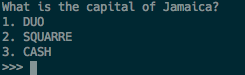
\includegraphics[scale=0.5]{choix}
      \caption{Exemple de choix de la méthode}
    \end{figure}
        \begin{itemize}
      \item Nombre de réponses limitées pour DUO
    \end{itemize}
    \begin{figure}[!b]
      \centering
      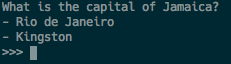
\includegraphics[scale=0.5]{reponse}
      \caption{Exemple de réponse}
    \end{figure}
  \end{frame}

  \begin{frame}{Conclusion (1)}
    \frametitle{Conclusion (1)}
    Le pattern stratégie est utilisé:
    \begin{itemize}
      \item Plusieurs choix possible par  \textcolor{red}{une classe utilisateur}\\
      \textit{Différents choix possibles pour l'utilisateurs. Exemple: proccèdure de réponses.}
      \item Une tâche se divise en  \textcolor{red}{plusieurs algorithmes} \\
      \textit{Exemple: Ajout de points en fonction d'un choix de réponse.}
    \end{itemize}
  \end{frame}
  
    \begin{frame}{Conclusion (2)}
    \frametitle{Conclusion (2)}
    Le pattern stratégie permet:
    \begin{itemize}
      \item Cacher \textcolor{red}{les details} d'implémentation \\
      \textit{Encapsulation des méthodes abstaites dans une interface.}
      \item Diviser une tâche en \textcolor{red}{plusieurs algorithmes} \\
      \textit{Différentes stratégies en fonction de certains paramêtres pour une tâche}
    \end{itemize}
  \end{frame}

  \appendix

  \begin{frame}{Enjoy!}
    The application burger is available on GitHub:
    \begin{itemize}
      \item \url{https://github.com/JonathanPetit/Strategy-design-pattern}
      \item Pour lancer l'application README.md
    \end{itemize}
  \end{frame}

  \begin{frame}[allowframebreaks]{Bibliography}
    \begin{thebibliography}{9}
      \setbeamertemplate{bibliography item}[online]
      \bibitem{A} \url{https://sourcemaking.com/design_patterns/strategy}
      \setbeamertemplate{bibliography item}[online]
      \bibitem{A} \url{https://medium.com/@sheikhsajid/design-patterns-in-python-part-1-the-strategy-pattern-54b24897233e}
      \setbeamertemplate{bibliography item}[online]
      \bibitem{A} \url{https://medium.com/@iimam/design-patterns-with-python-strategy-pattern-f4c076b5dd77}
      \setbeamertemplate{bibliography item}[book]
      \bibitem{B} Architecture logiciel slides - Mr. Comb\'efis
      \setbeamertemplate{bibliography item}[online]
      \bibitem{B} \url{https://github.com/matze/mtheme}

    \end{thebibliography}
  \end{frame}

\end{document}
